In the analyses discussed in this dissertation, smooth functional forms are used to model both the signal and background. This allows an unbinned likelihood fit to be performed, the preferable statistical analysis method in the lower-statistics $ttH$ regime (an alternative to the binned likelihood fit, also common in ATLAS analyses, which offers more statistics per bin, but a general loss of precision). 

Additionally, parameterizing signal and background in this way allows for the relatively straightforward calculation of several key systematics, including "spurious signal" background mismodelling, photon energy scale, and photon energy resolution.

\section{Signal Modelling} \label{sec:example_section} 

In collider physics analyses, one of the most common forms of signal is a "resonance", a bump in a smooth energy spectrum indicating the presence of a particle with mass given by the center of the resonance bump and lifetime given by the width $\Gamma$ of the resonance bump \cite{Peskin}. The "true underlying form" of resonances generally follow the Breit-Wigner distribution described in \cite{SlowNeutrons}; however, due to detector and beam effects, this form does not accurately describe observed data.

Instead, for both analyses discussed in this dissertation, a "Double-Sided Crystal Ball" (DSCB) function \cite{CB}\cite{DSCB} is used. The function has six parameters, two that describe the shape of its Gaussian core $\mu_{CB}$, and $\sigma_{CB}$, and two that describe the shape of each of its exponential tails: $\alpha_{low}$ and $n_{low}$; $\alpha_{high}$ and $n_{high}$. The function is defined as:

\[f_{DSCB}(m_{\gamma \gamma}) = \begin{cases} 
      e^{\frac{-{\alpha_{low}^{2}}}{2}} (\frac{R_{low}-\alpha_{low}-t}{R_{low}})^{n_{low}} & \mbox{if } t < -\alpha_{low} \\
      e^{\frac{-t^{2}}{2}} & \mbox{if } -\alpha_{low} \leq t \leq \alpha_{high} \\
      e^{\frac{-{\alpha_{high}^{2}}}{2}} (\frac{R_{high}-\alpha_{high}+t}{R_{high}})^{n_{high}} & \mbox{if } t > \alpha_{high} \\
   \end{cases}
\]

where $t = \frac{(m_{\gamma \gamma} - \mu_{CB})}{\sigma_{CB}}$ and $R = \frac{n}{\alpha}$. 

To parameterize the signal in each analysis category for both analyses discussed in this dissertation, all Monte Carlo for the various Higgs production modes ($VBF$, $VH$, $ggF$, $ttH$, $tWH$, $tHjb$ and $bbH$) generated using a Higgs mass of 125 GeV are combined. The resulting distribution is then fit with a DSCB function, and a rigid transformation of 0.09 GeV is performed such that the mean of the fitted DSCB corresponds to the experimentally measured Higgs mass of $125.09 GeV \pm 0.21 GeV(stat) \pm 0.1 GeV(syst)$ \cite{Higgsmass}.

Because the Double-Sided Crystal Ball function depends strongly on the photon resolution and energy scale, these systematics can be straightforwardly parameterized in the final fit as variations on $\mu_{CB}$ and $\sigma_{CB}$ \cite{gammaID}. This is one of the primary motivations for using this functional form, rather than a Gaussian or other distribution. Examples of DSCB shapes in five categories targeting two STXS truth bins of the Couplings Analysis are shown in Figure \ref{fig:DSCB}.

\begin{figure}[h]
\centering
\subfloat[$gg \rightarrow H$ ( 1-jet, $120 GeV \le p_{T}^{H} < 200 GeV$)] { 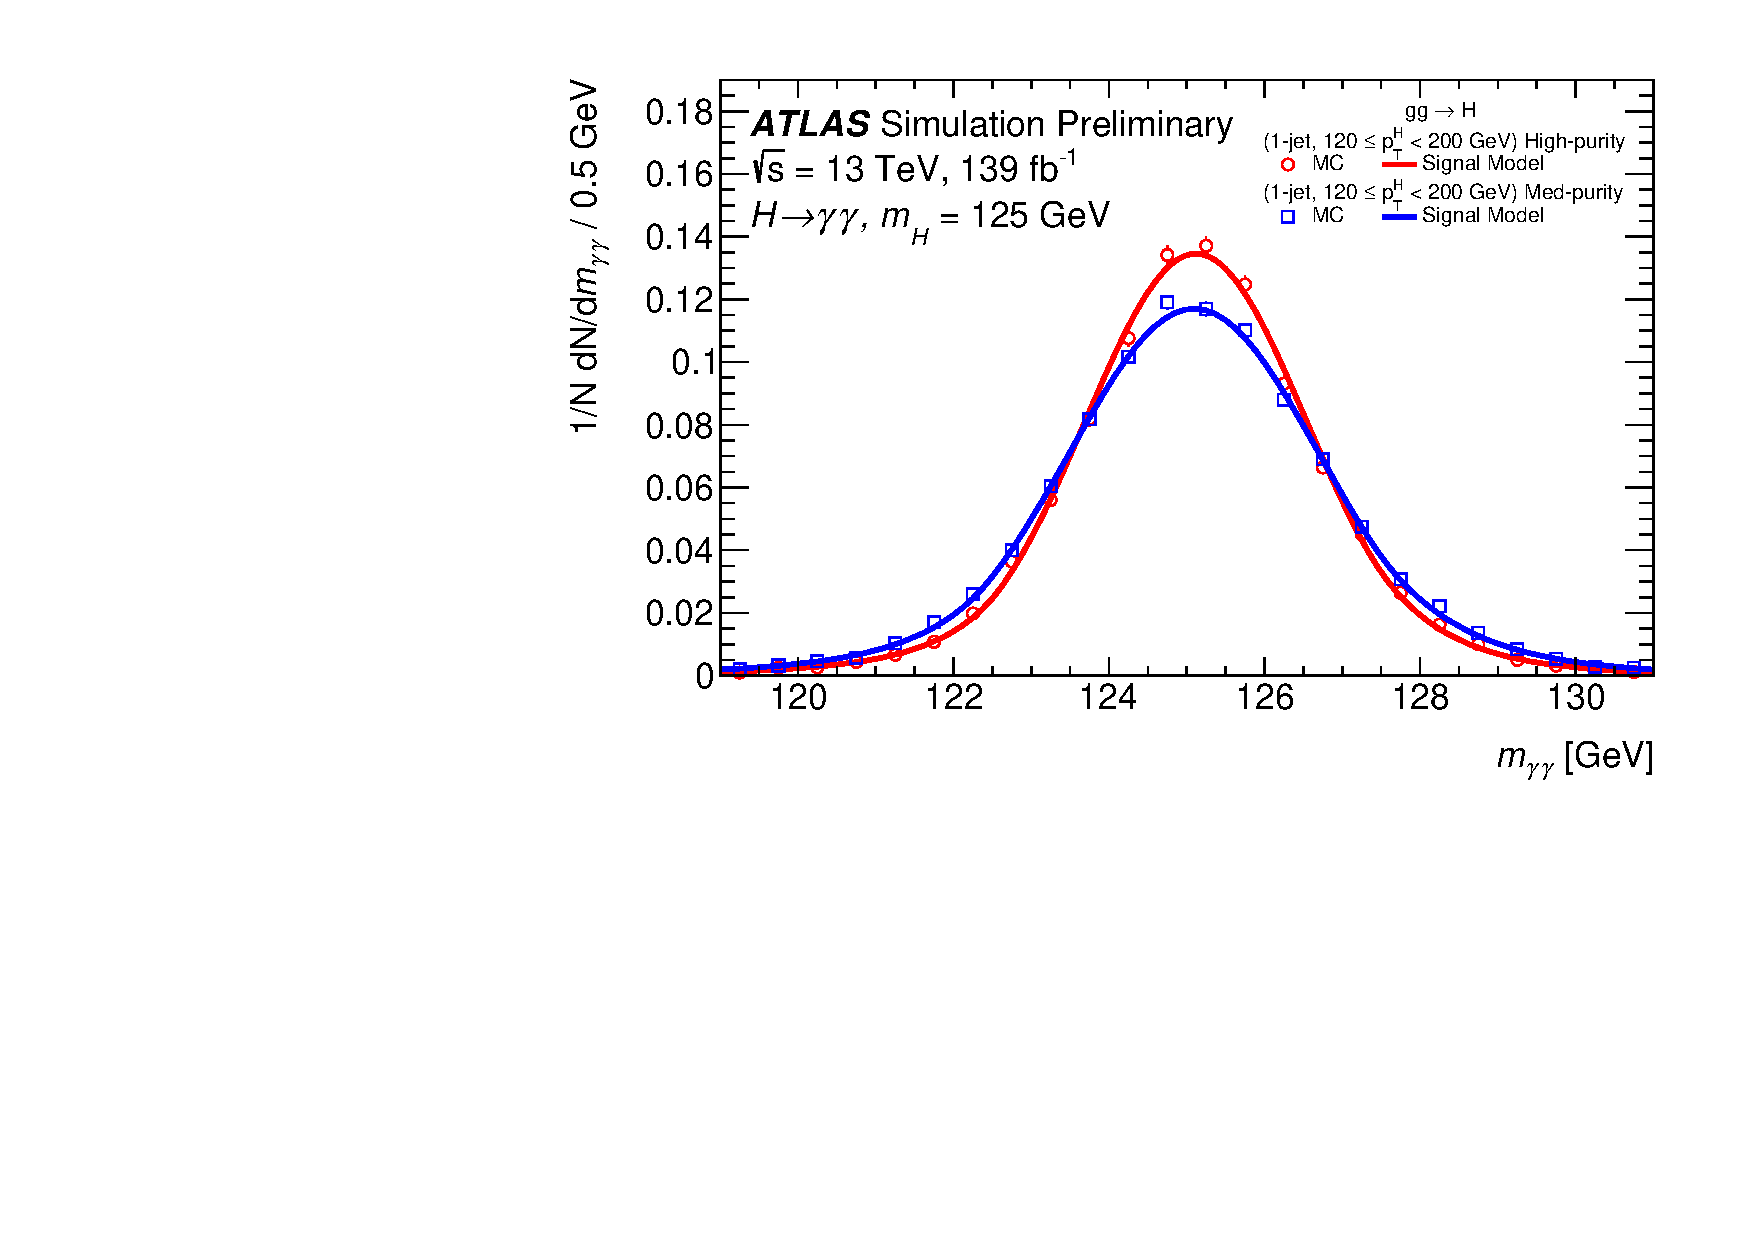
\includegraphics[width=0.49\textwidth]{figures/sigbkgparam/ggH_1J_120_200.pdf}\label{fig:DSCBgg2H}}
\subfloat[\ttH]{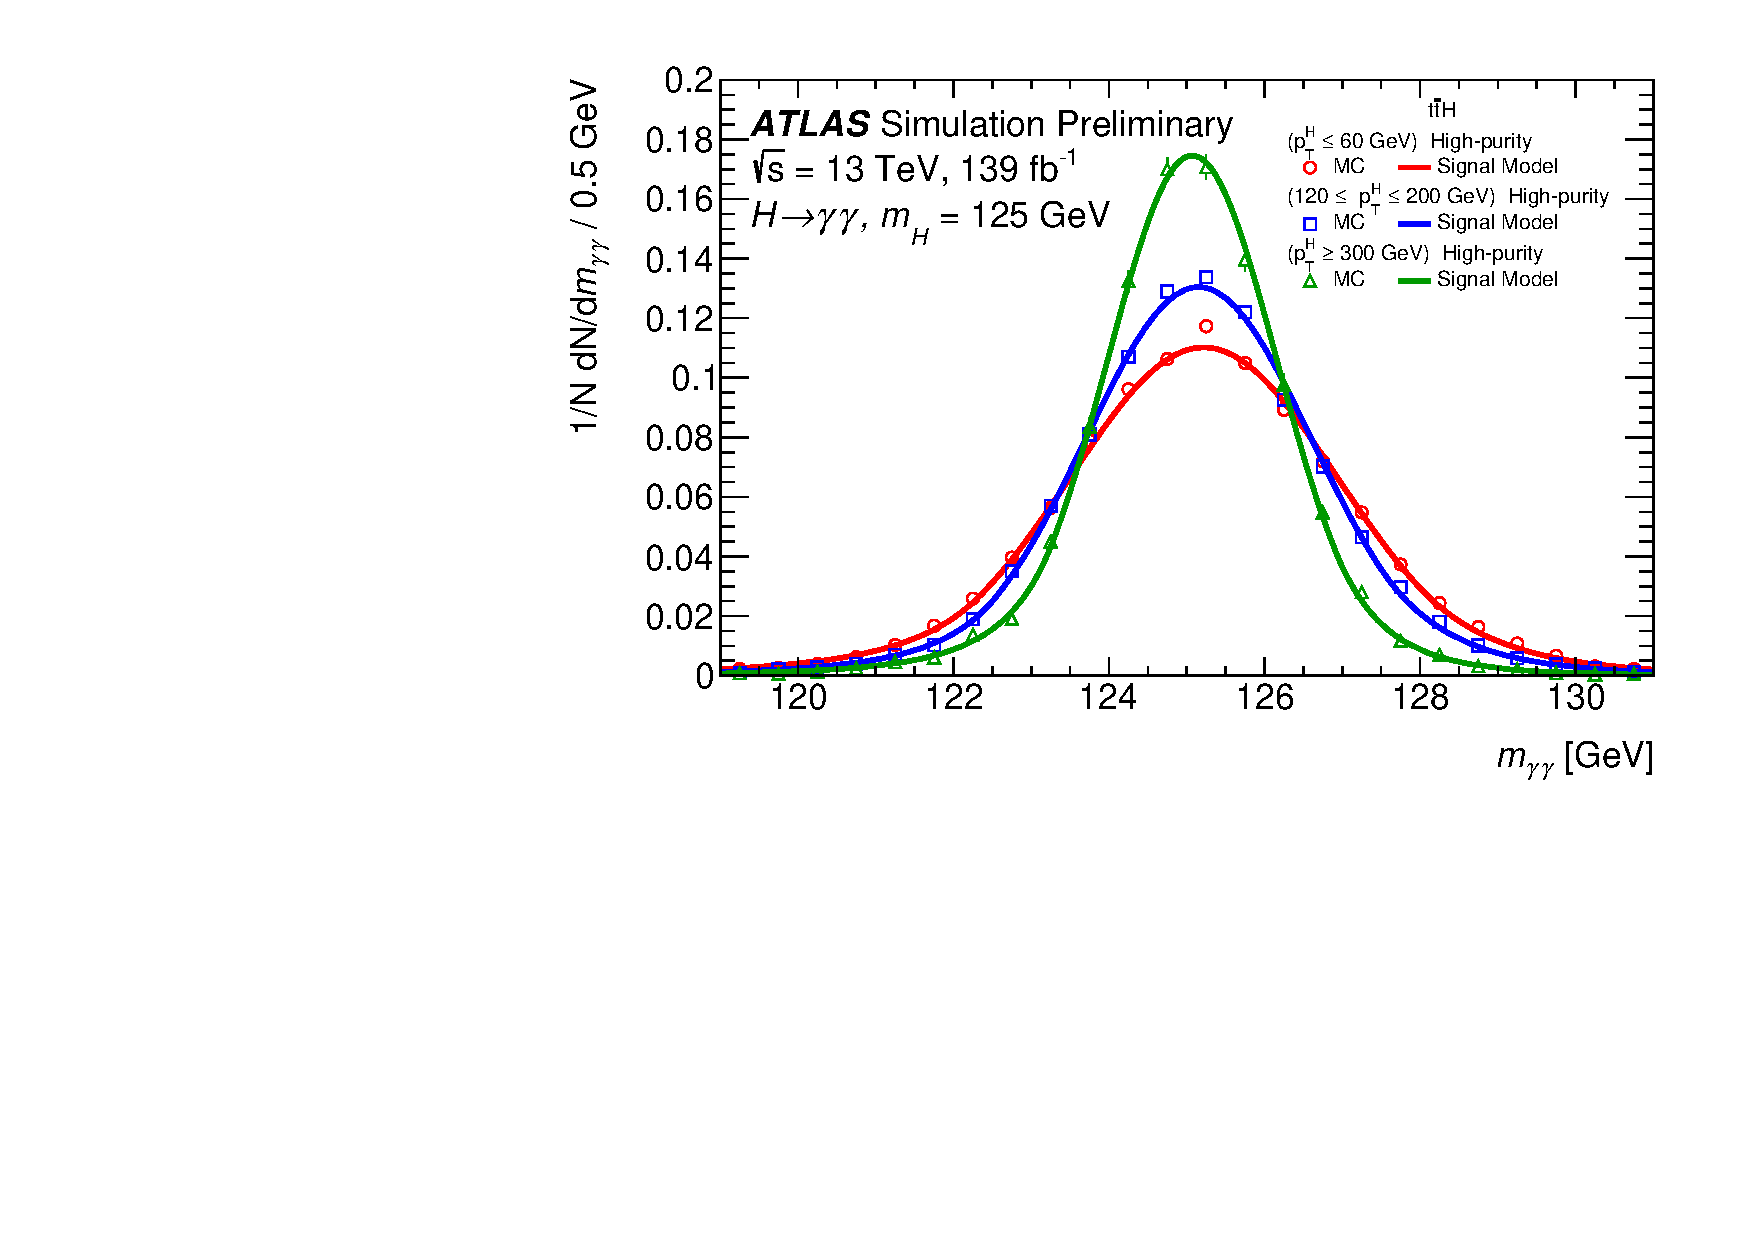
\includegraphics[width=0.49\textwidth]{figures/sigbkgparam/ttH.pdf}\label{fig:DSCBttH}}
\caption{DSCB shapes for two groups of categories. \ref{fig:DSCBgg2H} depicts the signal shapes for two categories targeting the same $ggH$ STXS truth bin, one low-purity and one high-purity. \ref{fig:DSCBttH} depicts the signal shapes for three high-purity categories targeting different $p_{T}^{H}$ regions of the $ttH$ process.}
\label{fig:DSCB}
\end{figure}

\section{Background Modelling and Spurious Signal} \label{sec:background_modelling} 

Like the signal, the background is also parameterized as a smoothly-falling functional form in each category. This is done in a data-driven manner: first, a functional form is chosen using simulation-derived (or NTI-derived) templates to minimize the "spurious signal" systematic uncertainty. The background normalization and parameters of this functional form are then allowed to float in the final fit to the data, i.e., they are not fixed as a result of the spurious signal test. 

Background templates for the spurious signal test are constructed from Monte Carlo or NTI data to resemble the expected TI data as closely as possible in each category. The construction of the templates is detailed further in section \label{sec:bkgtemplates}.

The spurious signal test is a signal-plus-background functional fit to a background-only distribution. This provides a relatively simple way to measure background mismodelling- the background template contains no true Higgs signal, so the functional form that best models the background is the one for which the extracted "spurious" signal is closest to zero. This is illustrated in figure \ref{fig:SScartoon}. Spurious signal can be positive or negative- if positive, the functional form chosen "undershoots" the true background, while if negative, the functional form chosen "overshoots" the true background.

\begin{figure}
\centering
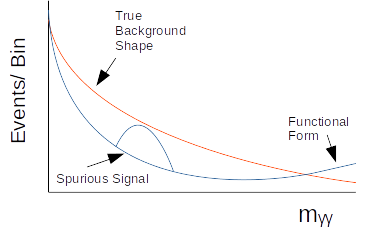
\includegraphics[width=0.49\textwidth]{figures/sigbkgparam/SSCartoon.png}
\caption{A cartoon depicting the spurious signal procedure. The true background shape in red is modeled by an analytic function in blue. The spurious signal resulting from this mismodelling is the maximum signal yield extracted from the blue "spurious signal" bump, fit over a window of $120 GeV < m_{\gamma \gamma}<130 GeV$.}
\label{fig:SScartoon}
\end{figure} 

The spurious signal fit is performed for signal masses from 121 GeV to 129 GeV at intervals of 1 GeV; the number of spurious signal events $N_{sp}$ is defined as the maximum of the absolute value of the number of signal events extracted from this range. The functional form chosen is one of the following functional forms:

\begin{itemize}
\item Exponential Function: $f(\myy) = e^{c\cdot \myy}$
\item Exponential Function of $2^{nd}$ Order Polynomial: $f(\myy) = e^{c_1\cdot m^2_{\gamma\gamma}+c_2\cdot \myy}$
\item Bernstein polynomial of order $N$: $B_{N}(\myy) = \sum_{i=0}^N c_i\cdot b_{i,N}$ with ${b_{i,N} = \begin{pmatrix}N\\i\end{pmatrix}\myy^i (1-\myy)^{N-i}}$
\item First-Order Power Law Function: $f(\myy) = \myy^c$
\end{itemize}

Functional forms chosen are then required to satisfy one of the two following criteria:

\begin{itemize}
\item $N_{s} < 0.1 \times N_{s,exp}$, where $N_{s,exp}$ is the expected true signal in a given category
\item $N_{s} < 0.2 \times \sigma_{s,exp}$, where $\sigma_{s,exp}$ is the statistical uncertainty on the expected true signal in a given category
\end{itemize}

If more than one function passes these criteria, the function with the lower number of degrees of freedom is selected. If there are multiple functions that pass the critera and have the same number of degrees of freedom, the function with the lowest resulting spurious signal is selected.

In low statistics categories, it is not uncommon that no functional form will satisfy the above criteria. In this case, the "relaxed" spurious signal fit is performed, which replaces $N_{s}$ with a new variable $\zeta_{s}$ that is designed to accomodate up to $2\sigma$ fluctuations in the spurious signal:

\[\zeta_{s} = \begin{cases} 
      N_{s} + 2 \delta_{MC} & \mbox{if }  N_{s} + 2 \delta_{MC} < 0\\
      N_{s} - 2 \delta_{MC} & \mbox{if }  N_{s} - 2 \delta_{MC} > 0\\
      0 & \mbox{otherwise } \\
   \end{cases}
\]

Though $\zeta_{s}$ is used to define the spurious signal criteria, $N_{s}$ is still used for the final spurious signal uncertainty. 

\begin{figure}
\centering
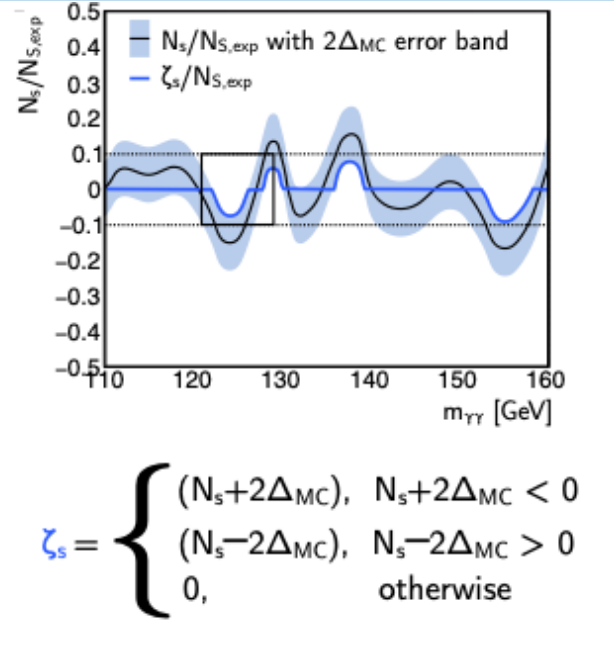
\includegraphics[width=0.49\textwidth]{figures/sigbkgparam/SSRelaxed.png}
\caption{A cartoon depicting the "relaxed" spurious signal procedure. Two-sigma fluctuations of the background are incorporated into the spurious signal procedure in order to select a functional form.}
\label{fig:SSrelaxed}
\end{figure} 


An additional requirement that the $\chi^{2}$ probability of the signal-plus-background fit in the spurious signal test is greater than 1\% is applied in the Couplings analysis; while this is not a requirement in the CP analysis, all sprurious signal fits nonetheless satisfy this criterion as well.

In the Couplings analysis, several of the very low-stat categories nevertheless produce unphysical fits using these criteria. Thus, in categories of this analysis containing fewer than 100 events in the data sidebands, a Wald test is performed: the functional forms are restricted to Exp, ExpPoly2, and ExpPoly3, and their respective maximum-likelihoods $L_{1}$, $L_{2}$, and $L_{3}$ are computed from a fit to the TI data sidebands. The quantities $q_{ij} = -2 ln(\frac{L_{i}}{L_{j}})$ are then calculated and converted into p-values, assuming that $q_{ij}$ follows a $\chi^{2}$ distribution with one degree of freedom. If the p-value calculated is < 0.05, the function with the larger number of degrees of freedom is chosen. 

An illustration of the Wald test in two of the Couplings categories is shown in Figure \ref{fig:WaldTest}.

\begin{figure}
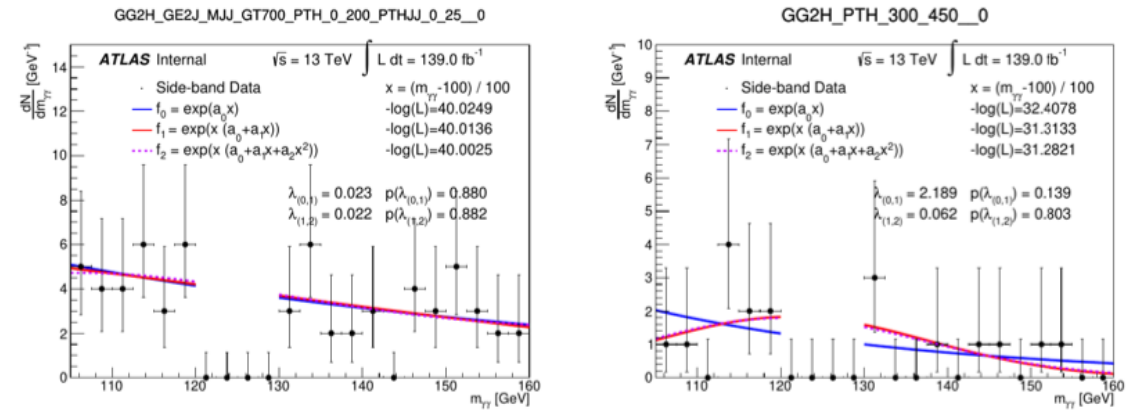
\includegraphics[width=\linewidth]{figures/sigbkgparam/Walds.png}
\caption{An example of the Wald test being performed in two low-statistics Couplings categories. The exponential functional form is chosen in both cases.}
\label{fig:WaldTest}
\end{figure} 

These failed fits show the limitations of current spurious signal criteria: in low-statistics categories, the Monte Carlo templates often contain large statistical fluctuations that can be fit as spurious signal. However, because spurious signal is intended to measure the mismodelling due to the choice of functional form, the presence of such fluctuations can artifically inflate the spurious signal. If the functional forms chosen because of these fluctuations have too many degrees of freedom, this can cause disastrous effects when fitting to the true data sidebands, as statistical fluctuations in data will dominate. This is the motivation for introducing Gaussian Process Regression (GPR) smoothing, discussed in appendix \ref{app:gpr_templates}. At the time of this writing, this novel smoothing procedure is currently being implemented in the Couplings analysis; a discussion of the procedure and the improvements to the spurious signal that result are given in appendix \ref{app:gpr_templates}, while extensive validation of the smoothing procedure using toy tests is given in appendix \ref{app:gpr_validation}.

\subsubsection{Background Templates} \label{sec:bkgtemplates} 

The background templates constructed for both analyses discussed in this dissertation are designed to approximate the continuum diphoton background. 

In all categories of the CP analysis, either $tt\gamma\gamma$ Monte Carlo or NTI data is used to model the continuum background, scaled to the TI data sidebands. The statistical uncertainty of both template candidates is checked in each region by taking the integral and sum of errors; the template chosen is the one with the smallest statistical uncertainty. $tt\gamma\gamma$ is ultimately used to construct the template in all CP analysis categories but one. 

Similarly, in the leptonic $VH$ categories of the Coupling analysis, a combination of $\gamma\gamma + V\gamma\gamma$ Monte Carlo, scaled to match the TI sidebands, is used. However, in the other $ggH$ and $VBF$ categories, a more sophisticated data-driven method is used due to the nontrivial presence of fake photons arising from misidentified jets. 

First, the purity fraction, i.e. the fraction of true vs. fake diphoton events in data, is calculated in each category. This is done using a double two-dimensional ABCD method \cite{purity1} \cite{purity2}.

For a given choice of photon (either leading or subleading) four regions are constructed in each category:

\begin{itemize}
\item Region A, in which the photon passes the Tight ID criterion and the Tight isolation criterion
\item Region B, which the photon passes the Tight ID criterion and fails the Tight isolation criterion
\item Region C, in which the photon fails the Tight ID criterion (but passes the LoosePrime3 ID criterion) and fail the Tight isolation criterion
\item Region D, in which the photon fails the Tight ID criterion (but passes the LoosePrime3 ID criterion) and passes the Tight isolation criterion
\end{itemize} 

Assuming that the ID and isolation cuts are independent with $\epsilon_{ID}$ and $\epsilon_{iso}$, and that the photons in all regions but region A are definitively fakes, it is possible to define the number of fake photons in region A as:

\begin{equation}
N_{A} = \epsilon_{iso} N_{B} = \epsilon_{ID} N_{D} = \epsilon_{iso} \epsilon_{ID} N_{C}
\end{equation} 

Extending this to the diphoton pair, eight total regions can be defined in each category, allowing us to quantify the ($\gamma \gamma / \gamma j/jj$) fraction in each category. However, the assumption that the isolation and ID cuts are independent is not strictly valid, so it is not enough to perform a simple counting-experiment to determine the fraction of jets: various correlation terms must be considered, so a fit must be performed. The fit has sixteen equations with nineteen variables, and is performed following the process in \cite{purity1} and \cite{purity2}.

After the purity fractions are calculated in each category, the shapes of the $\gamma j$ and $jj$ distributions are derived using NTI data. The $\gamma \gamma$ Monte Carlo is then reweighted to match these shapes, and the $\gamma \gamma$, $\gamma j$, and $jj$ contributions are added according to their purities. As in other categories, the templates are scaled to the TI sidebands. 

\subsection{The Kappa Framework} \label{sec:kappaFW}

When measuring Higgs couplings in ATLAS, it is often more useful to note the ratio of the measured coupling to the Standard Model prediction rather than the measured coupling alone. For some Higgs coupling to a boson or fermion $i$, we can write

\begin{equation}
\kappa_{i} = \frac{y_{i}^{meas}}{y_{i}^{SM}}
\end{equation}

This $\kappa$ parameter is called the "coupling strength"-- if $\kappa_{i} = 1$, the Higgs couples to particle $i$ exactly as predicted by the Standard Model, while if $\kappa_{i} = 0$, the Higgs does not couple to particle $i$ at all. Measuring the Higgs couplings and interactions in this manner is referred to as the "Kappa Framework" \cite{LHCHiggsCrossSectionWorkingGroup}.

The parameterization of various production cross-sections and decay widths (divided by their Standard Model values) in terms of the $\kappa$ framework is shown in Tables \ref{tab:Xsecskappa}-\ref{tab:BRskappa} \cite{PhysRevD.101.012002}. The "resolved" column assumes that only the particles of the Standard Model exist. However, it can also be useful to develop "effective" coupling terms that allows for the existence of additional particles that may influence the loop diagrams. These can be modeled by mutiplying the resolved coupling terms by the indicated factors:

\begin{equation}
\kappa_{g}^{2} = \frac{\sigma_{ggF}^{meas}}{\sigma_{ggF}^{SM}}, \kappa_{\gamma}^{2} = \frac{\Gamma{\gamma \gamma}^{meas}}{\Gamma_{\gamma \gamma}^{SM}}, \kappa_{Z \gamma}^{2} = \frac{\Gamma{Z \gamma}^{meas}}{\Gamma_{Z \gamma}^{SM}}
\end{equation}

\begin{table}[h]
    \centering
    \begin{tabular}{ccc}
	Production Mode & Effective Modifier & Resolved Modifier \\ \hline
	$\sigma(ggF)$ & $\kappa_{g}^{2}$ & $1.04 \kappa_{t}^{2} + 0.002 \kappa_{b}^2 - 0.04 \kappa_{t} \kappa_{b}$ \\
	$\sigma(VBF)$ & & $0.73 \kappa_{W}^{2} + 0.27 \kappa_{Z}^2$ \\
	$\sigma(qq/qg \rightarrow W H)$ & & $\kappa_{W}^{2}$ \\
	$\sigma(qq/qg \rightarrow ZH)$ & & $\kappa_{Z}^{2}$\\
	$\sigma(ggZH)$ && $2.46 \kappa_{Z}^{2} + 0.46 \kappa_{t}^2 - 1.90 \kappa_{t} \kappa_{Z}$ \\
	$\sigma(t\bar{t}H)$ && $\kappa_{t}^{2}$ \\
	$\sigma(b\bar{b}H)$ && $\kappa_{b}^{2}$ \\
	$\sigma(tHjb)$ && $2.63 \kappa_{t}^{2} + 3.58 \kappa_{W}^2 - 5.21 \kappa_{t} \kappa_{W}$ \\
	$\sigma(tWH)$ && $2.91 \kappa_{t}^{2} + 2.31 \kappa_{W}^2 - 4.22 \kappa_{t} \kappa_{W}$ \\
    \end{tabular}
    \caption{Parameterization of Higgs cross-section dependence on $\kappa$ coefficients, from \cite{PhysRevD.101.012002}}
    \label{tab:Xsecskappa}
\end{table}

\begin{table}[h]
    \centering
    \begin{tabular}{ccc}
	Production Mode & Effective Modifier & Resolved Modifier \\ \hline
	$H \rightarrow bb$ & & $\kappa_{b}^2$ \\
	$H \rightarrow WW$ & & $\kappa_{W}^{2}$ \\
	$H \rightarrow gg$ & $\kappa_{g}^{2}$ & $1.11 \kappa_{t}^{2} + 0.01 \kappa_{b}^2 - 0.12 \kappa_{t} \kappa_{b}$ \\
	$H \rightarrow \tau \tau$ & & $\kappa_{\tau}^{2}$ \\
	$H \rightarrow cc$ && $2.46 \kappa_{c}^{2}$ \\
	$H \rightarrow ZZ$ && $\kappa_{Z}^{2}$ \\
	$H \rightarrow \gamma \gamma$ & $\kappa_{\gamma}^{2}$ & $1.59 \kappa_{W}^{2} + 0.07 \kappa_{t}^2 - 0.67 \kappa_{t} \kappa_{W}$ \\
	$H \rightarrow Z \gamma$ & $\kappa_{z \gamma}^{2}$ & $1.12 \kappa_{W}^{2} + 0.12 \kappa_{t} \kappa_{W}$ \\
	$H \rightarrow \mu \mu$ && $\kappa_{\mu}^{2}$ \\
    \end{tabular}
    \caption{Parameterization of Higgs branching ratio dependence on $\kappa$ coefficients, from \cite{PhysRevD.101.012002}}
    \label{tab:BRskappa}
\end{table}

\subsection{Simplified Template Cross-Sections} \label{sec:STXS}

The Couplings Analysis is performed within the Simplified Template Cross Sections (STXS 1.2) framework \cite{YellowReport4}, where different regions of phase space called "truth bins" are probed according to their production modes and kinematic properties. A visual guide to the different STXS1.2 bins is shown in figure \ref{fig:STXS_scheme}. The categorization is designed such that all events passing the $H \rightarrow \gamma \gamma$ selection criteria will fall into one of the STXS1.2 categories.

\begin{figure}[tbp]
  \centering
  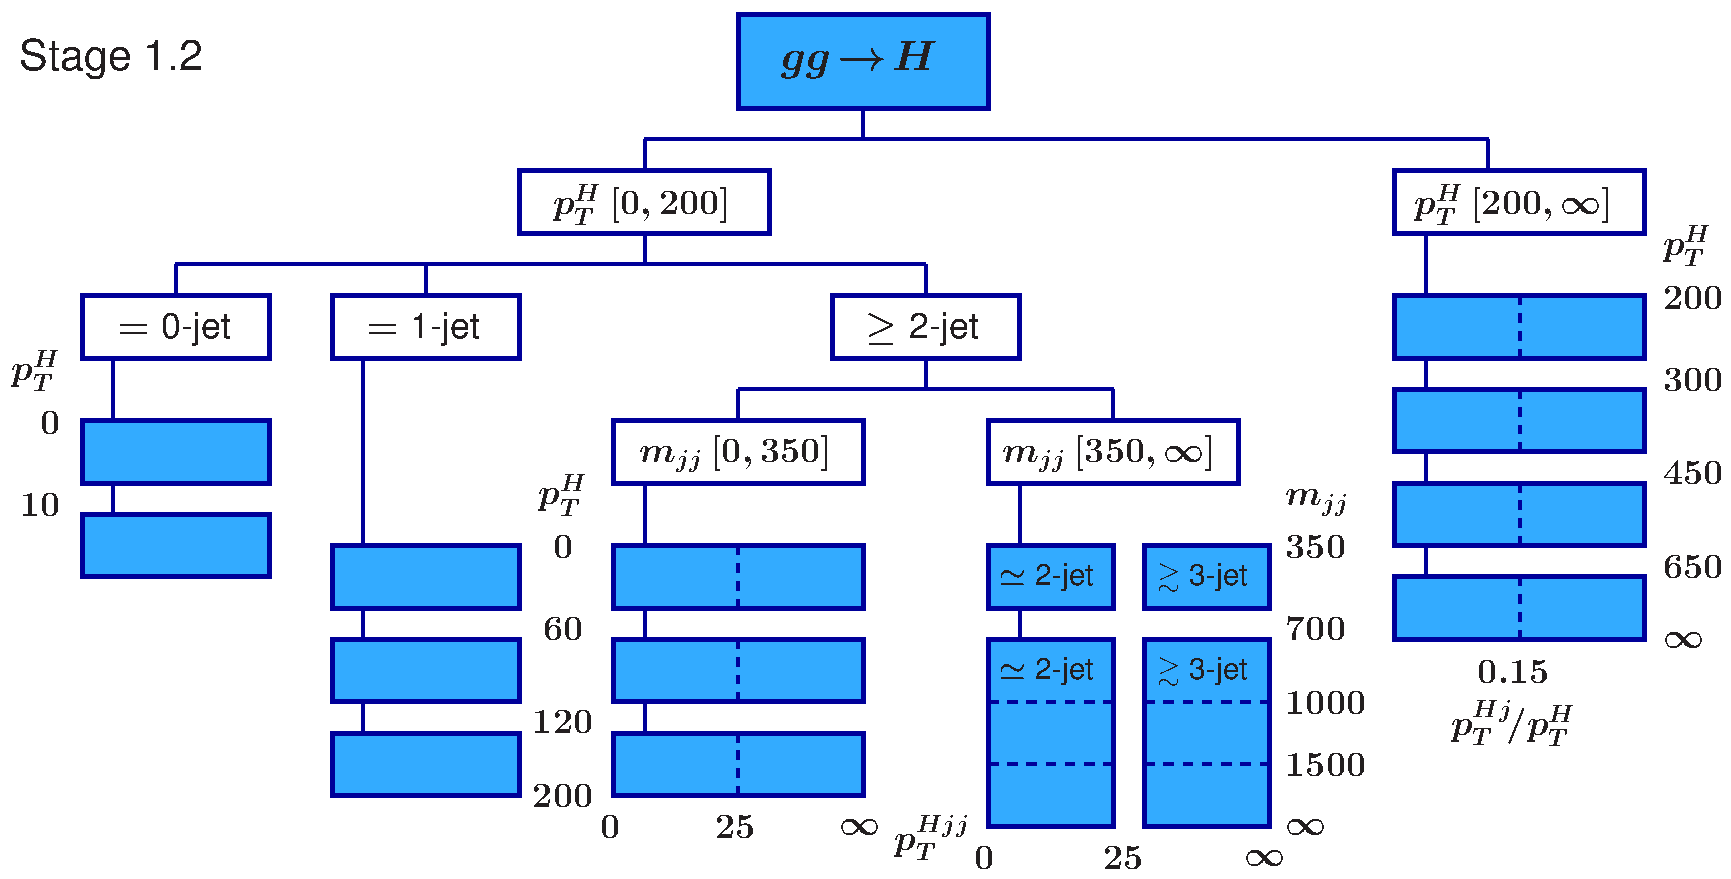
\includegraphics[width=0.8\textwidth]{figures/theory_chapter/simplifiedXS_ggF_1_2} \\[3mm]
  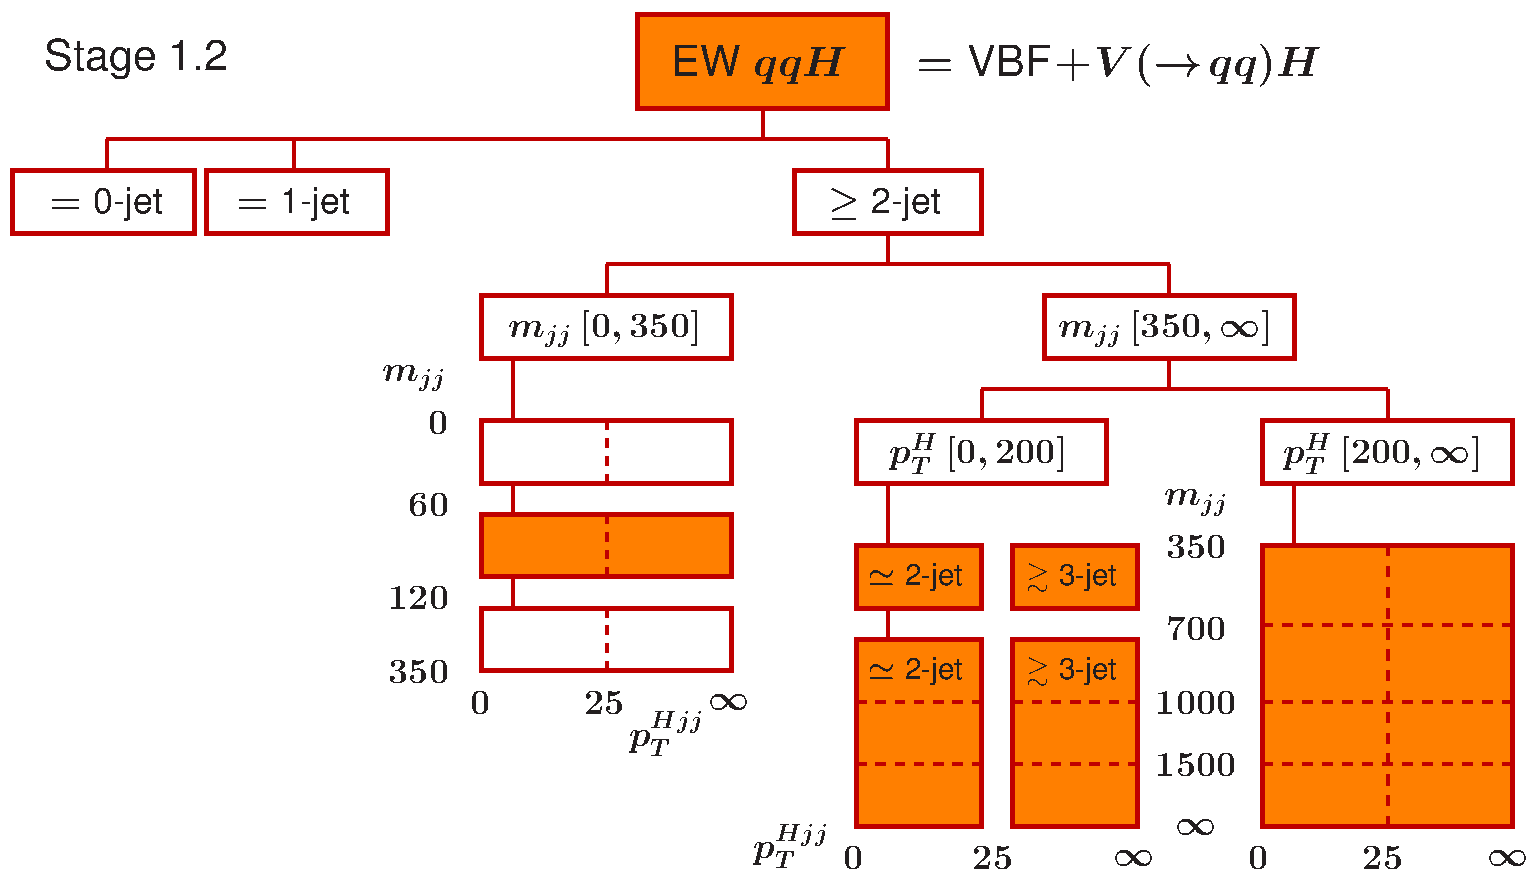
\includegraphics[width=0.8\textwidth]{figures/theory_chapter/simplifiedXS_VBF_1_2} \\[3mm]
  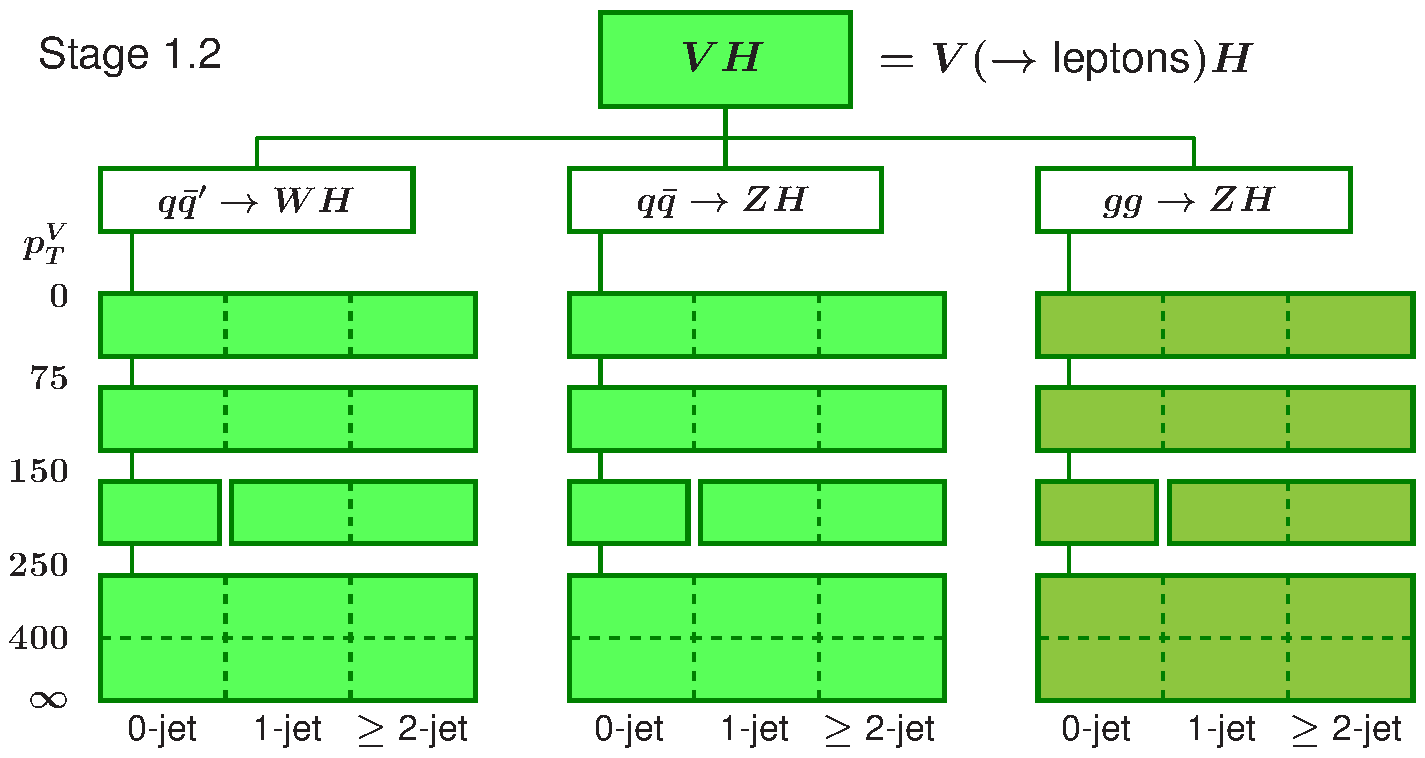
\includegraphics[width=0.6\textwidth]{figures/theory_chapter/simplifiedXS_VH_1_2}
  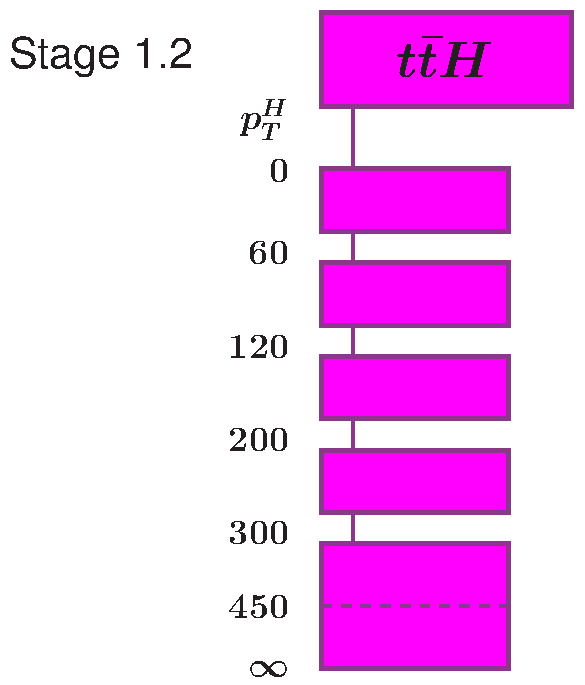
\includegraphics[width=0.25\textwidth]{figures/theory_chapter/simplifiedXS_ttH_1_2}
  \caption{Stage 1.2 STXS bin definitions for the main production modes.}
  \label{fig:STXS_scheme}
\end{figure}


In addition to their nominal production and decay modes, the $ggH$ STXS1.2 truth bins include both $ggF$ and hadronically-decaying $gg \rightarrow ZH$ events, while the $VBF$ STXS definition includes hadronically-decaying $qq \rightarrow VH$. Additionally, it is important to note that the leptonic $qq \rightarrow ZH$ and $gg \rightarrow ZH$ truth bins include Z-boson decays both to two charged leptons and to two neutrinos (the latter of which will have a high $E_T^{miss}$ signature). For nomenclature purposes, throughout this dissertation, $ggF$ is used to refer to the $gg \rightarrow H$ production mode, while $ggH$ is used to refer to the regions of phase space targeting the combination of $gg \rightarrow H$ and $gg \rightarrow ZH$.

In the Couplings analysis, the experimental bins targeted are modified somewhat from the truth bins due to the inability to separate some processes: the $b\bar{b}H$ categories are subsumed into the $ggH$ categorization scheme, the leptonic $qq \rightarrow VH$ and $gg \rightarrow VH$ processes are combined into a series of $VHLep$ regions, $tH$ is split into $tWH$ and $tHjb$, and the $p_{T}^H > 200$ GeV bin of the hadronic $qq \rightarrow VH$ truth category is split into two bins based on jet kinematics to aid in statistical combination with other analyses (where $p_{T}^{H}$ denotes the transverse momentum of the Higgs, that is, the component of the Higgs momentum perpendicular to the beamline). A total of 44 STXS truth regions are defined.

For all Monte Carlo simulated samples used to construct the STXS truth bins, the absolute value of the rapidity of the Higgs boson is required to satisfy $|y_{H}| < 2.5$ while jets, built with the anti-kT algorithm \cite{antikt} using radius R=0.4, are required to have $p_{T} > 30$ GeV (with the exception of the bins labelled FWDH, which target forward Higgs events with $|y_{H}| > 2.5$.

Using the Monte Carlo simulated samples described in section \ref{chap:datamc_chapter}, we report the cross-section times branching ratio and acceptances (in terms of percentage of events of each production-mode) that fall into each STXS1.2 truth bin in Table \ref{tab:STXS_cross_sections}, and show the acceptance for each production mode in Figure \ref{fig:STXS_acceptances}. Several of the STXS truth bins are merged in the Couplings analysis to account for effects such as the inability of the event classifier to discriminate between $qq \rightarrow ZH$ and $gg \rightarrow ZH$; this is detailed in section \ref{chap:couplings_chapter}. By measuring the cross-sections in each of these bins, a number of different values are able to be extracted, including the various Higgs couplings $\kappa$ and limits on effective field theories (EFTs) parameterizing physics beyond the standard model.

\begin{table}[htbp]
        \centering
        {\footnotesize
        \begin{tabular}{lS}
                STXS 1.2 Truth Bin                                     & {$\sigma\times BR_{\gamma \gamma} [\si{\fb}]$} \\
                \hline
                gg2H\_0J\_ptH\_0\_10                                   & 15.038147                                    \\
                gg2H\_0J\_ptH\_gt10                                    & 46.799419                                    \\
                gg2H\_1J\_ptH\_0\_60                                   & 14.742653                                    \\
                gg2H\_1J\_ptH\_60\_120                                 & 10.223149                                    \\
                gg2H\_1J\_ptH\_120\_200                                & 1.692748                                     \\
                gg2H\_ge2J\_MJJ\_0\_350\_ptH\_0\_60                    & 2.639954                                     \\
                gg2H\_ge2J\_MJJ\_0\_350\_ptH\_60\_120                  & 4.058768                                     \\
                gg2H\_ge2J\_MJJ\_0\_350\_ptH\_120\_200                 & 2.133361                                     \\
                gg2H\_ge2J\_MJJ\_350\_700\_ptH\_0\_200\_ptHJJ\_0\_25   & 0.569488                                     \\
                gg2H\_ge2J\_MJJ\_350\_700\_ptH\_0\_200\_ptHJJ\_gt25    & 0.818394                                     \\
                gg2H\_ge2J\_MJJ\_gt700\_ptH\_0\_200\_ptHJJ\_0\_25      & 0.241653                                     \\
                gg2H\_ge2J\_MJJ\_gt700\_ptH\_0\_200\_ptHJJ\_gt25       & 0.363737                                     \\
                gg2H\_ptH\_200\_300                                    & 1.036991                                     \\
                gg2H\_ptH\_300\_450                                    & 0.239097                                     \\
                gg2H\_ptH\_450\_650                                    & 0.035624                                     \\
                gg2H\_ptH\_gt650                                       & 0.004947                                     \\
                qq2Hqq\_0J                                             & 0.816245                                     \\
                qq2Hqq\_1J                                             & 3.956656                                     \\
                qq2Hqq\_ge2J\_MJJ\_0\_60                               & 0.224649                                     \\
                qq2Hqq\_ge2J\_MJJ\_60\_120                             & 1.200933                                     \\
                qq2Hqq\_ge2J\_MJJ\_120\_350                            & 1.426903                                     \\
                qq2Hqq\_ge2J\_MJJ\_350\_700\_ptH\_0\_200\_ptHJJ\_0\_25 & 0.897833                                     \\
                qq2Hqq\_ge2J\_MJJ\_350\_700\_ptH\_0\_200\_ptHJJ\_gt25  & 0.337811                                     \\
                qq2Hqq\_ge2J\_MJJ\_gt700\_ptH\_0\_200\_ptHJJ\_0\_25    & 1.356668                                     \\
                qq2Hqq\_ge2J\_MJJ\_gt700\_ptH\_0\_200\_ptHJJ\_gt25     & 0.314044                                     \\
                qq2Hqq\_ge2J\_MJJ\_350\_700\_ptH\_gt200                & 0.104740                                     \\
                qq2Hqq\_ge2J\_MJJ\_gt700\_ptH\_gt200                   & 0.258838                                     \\
                qq2Hlnu\_ptV\_0\_75                                    & 0.466795                                     \\
                qq2Hlnu\_ptV\_75\_150                                  & 0.297442                                     \\
                qq2Hlnu\_ptV\_150\_250\_0J                             & 0.051545                                     \\
                qq2Hlnu\_ptV\_150\_250\_ge1J                           & 0.042651                                     \\
                qq2Hlnu\_ptV\_gt250                                    & 0.030152                                     \\
                qq2Hll\_ptV\_0\_75                                     & 0.236572                                     \\
                qq2Hll\_ptV\_75\_150                                   & 0.157167                                     \\
                qq2Hll\_ptV\_150\_250\_0J                              & 0.027476                                     \\
                qq2Hll\_ptV\_150\_250\_ge1J                            & 0.022523                                     \\
                qq2Hll\_ptV\_gt250                                     & 0.015076                                     \\
                gg2Hll\_ptV\_0\_75                                     & 0.014989                                     \\
                gg2Hll\_ptV\_75\_150                                   & 0.038219                                     \\
                gg2Hll\_ptV\_150\_250\_0J                              & 0.007812                                     \\
                gg2Hll\_ptV\_150\_250\_ge1J                            & 0.014855                                     \\
                gg2Hll\_ptV\_gt250                                     & 0.004465                                     \\
                ttH\_ptH\_0\_60                                        & 0.267960                                     \\
                ttH\_ptH\_60\_120                                      & 0.404152                                     \\
                ttH\_ptH\_120\_200                                     & 0.287483                                     \\
                ttH\_ptH\_200\_300                                     & 0.119454                                     \\
                ttH\_ptH\_gt300                                        & 0.055617                                     \\
                bbH                                                    & 1.044426                                     \\
                tH                                                     & 0.187064                                     \\
                \hline
        \end{tabular}
        }
        \caption{Simplified template cross sections times diphoton branching ratio for each of the STXS 1.2 truth bins.}
        \label{tab:STXS_cross_sections}
\end{table}

\begin{figure}[tbp]
        \centering
        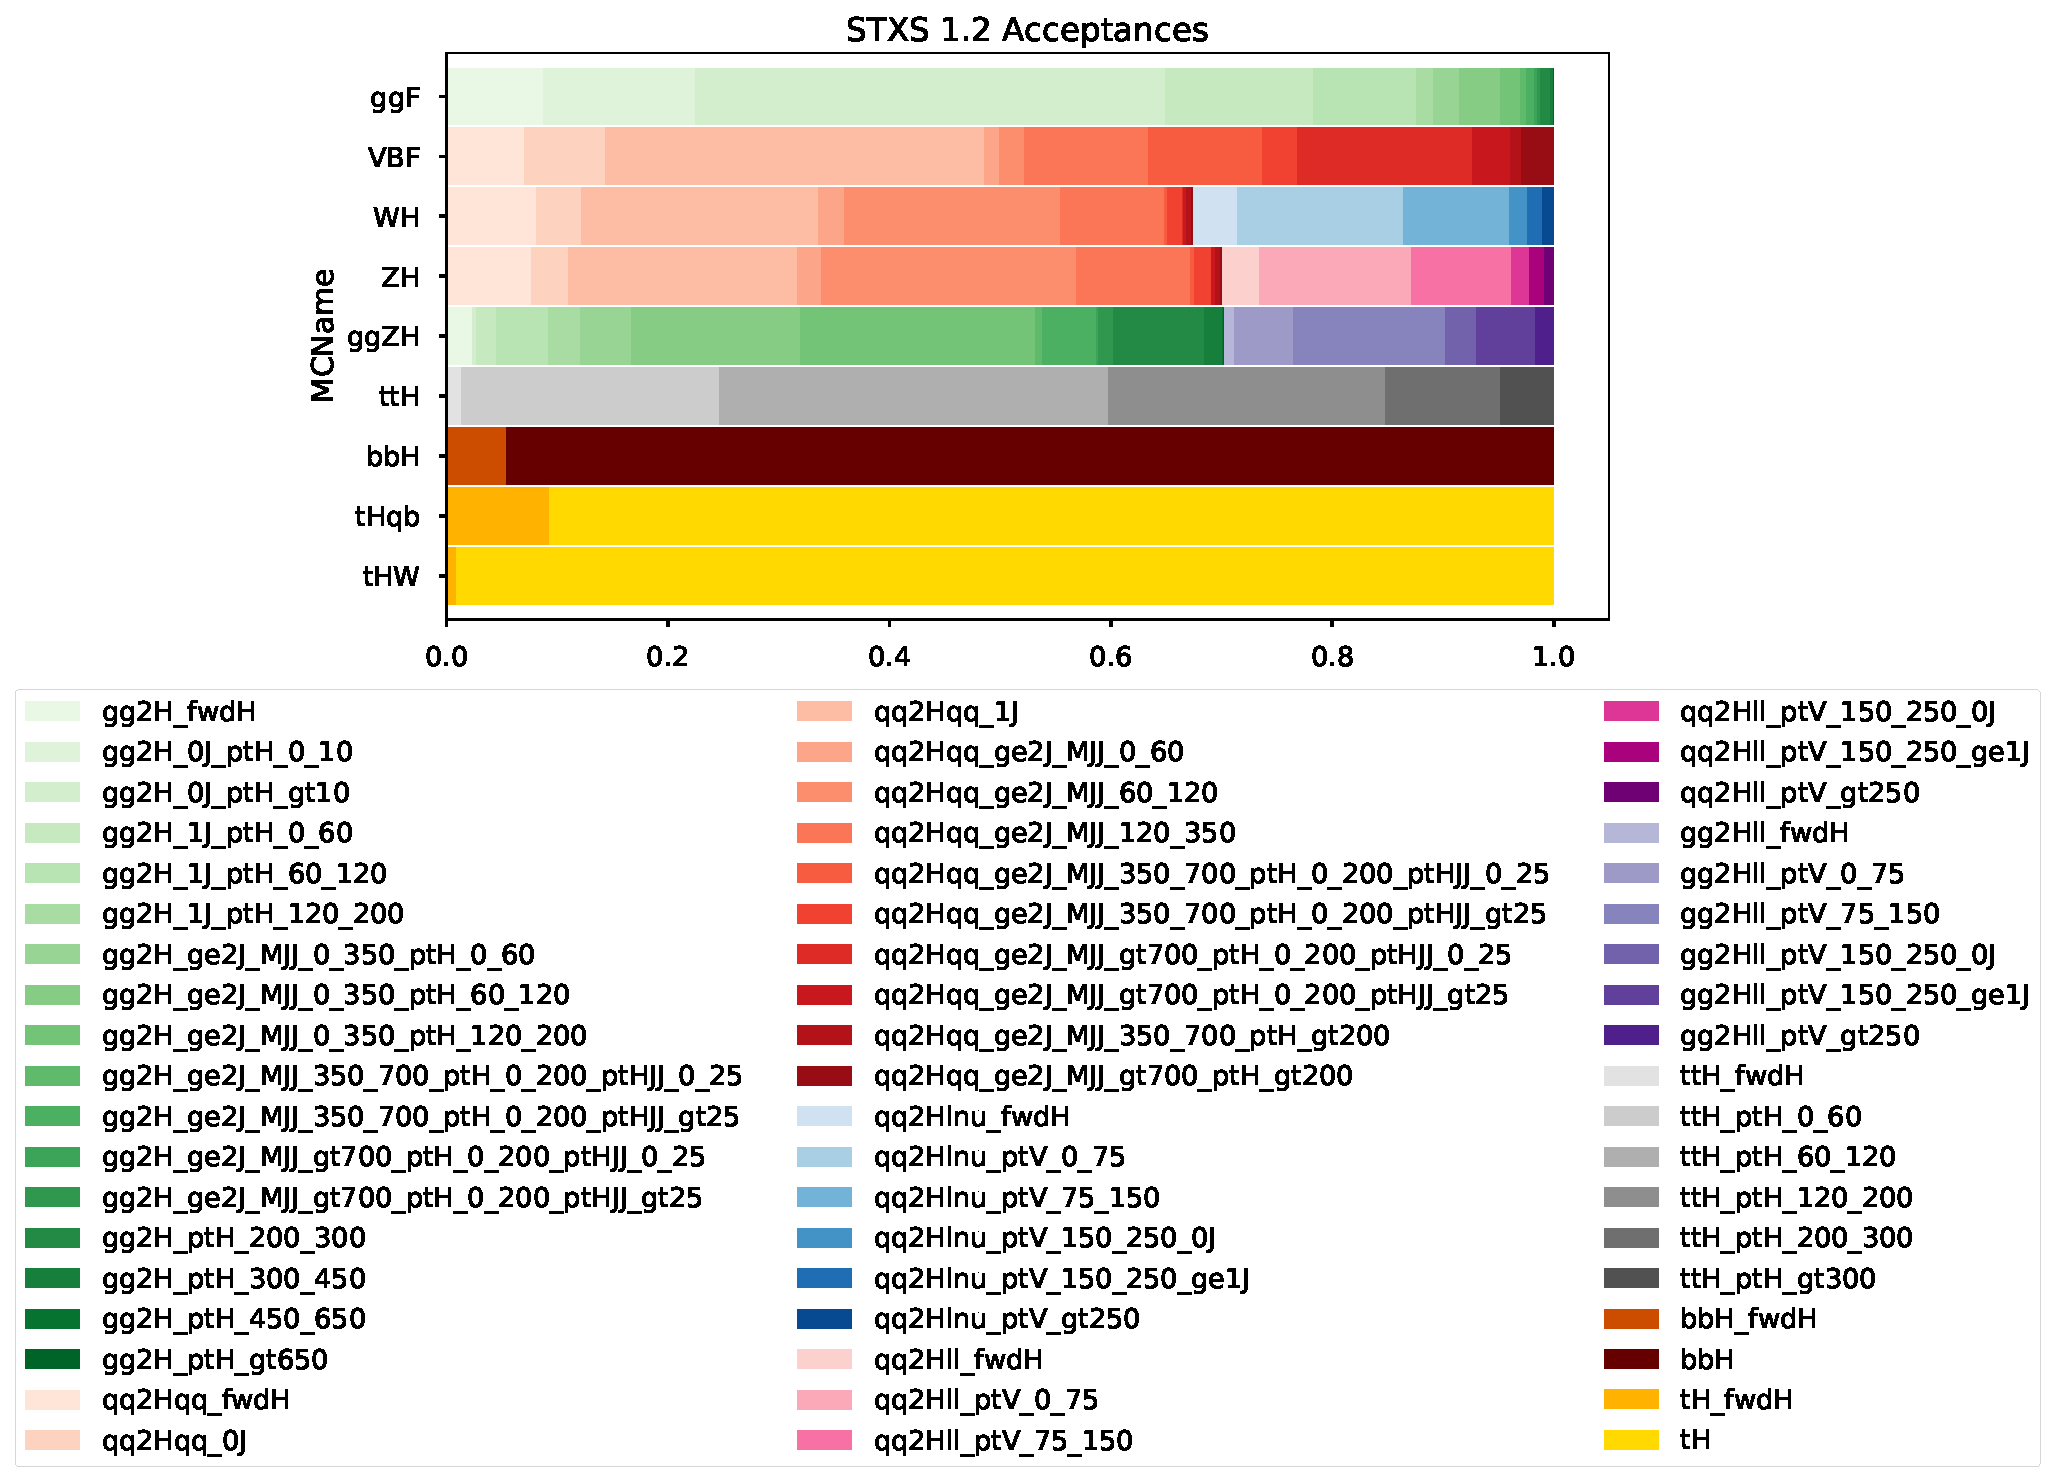
\includegraphics[width=\linewidth]{figures/theory_chapter/STXS_acceptances.pdf}
        \caption{Stage 1.2 STXS bin acceptances for all Higgs production modes considered in the Couplings analysis. The FWDH bins target events outside the nominal acceptance, i.e. with $|y_{H}|>2.5$.}
        \label{fig:STXS_acceptances}
\end{figure}

\section{Likelihood Fitting and Asimov Data} \label{sec:likelihoodfit} 

The fits performed in all analyses discussed in this dissertation use a test statistic called a Profile Likelihood Ratio. The likelihood ratio  is a Bayesian variable that is simply defined as $\mathcal{L}(\vec{x},\vec{\theta}) = P(\vec{x} | \vec{\theta})$  for a set of observed data points $\vec{x}$ and a set of additional nuisance-parameter variables $\vec{\theta}$ such as background normalization, shape, and systematic uncertainties \cite{Cowan}.

For independent, identically distributed Poisson variables (i.e., the number of signal and background events in a given histogram bin $i$), we can parameterize the likelihood as:

\begin{equation}
\mathcal{L}(\mu, N_{b}, \vec{\zeta}) = \prod_{i}^{N}{\frac{(\mu \times s_{i}+ N_{b} \times b_{i}(\vec(\zeta)))^{n_{i}} \times e^{-(\mu \times s_{i}+ N_{b} \times b_{i}(\vec(\zeta))) }}{n_{i}!}}
\end{equation}

for signal strength $\mu$, expected signal and background probability distributions $s_{i}$ and $b_{i}$ in each bin, nuisance parameters $\vec{\theta} = (N_{b}, \vec{\zeta})$ governing the total background normalization and shape, and $n_{i}$ observed number of events in bin i. Likelihoods can also be constructed in an unbinned manner by taking the continuous form of $s_{i}$ and $b_{i}$ as a function of $m_{\gamma\gamma}$. For a multi-category analysis, the total likelihood is taken as the product of the likelihood in each category.

Using this, we can construct the Profile Likelihood Ratio as: 
\begin{equation}
\lambda(\mu) = \frac{\mathcal{L}(\mu, \hat{\hat{\theta}}(\mu))} {\mathcal{L}(\hat{\mu}, \hat{\theta}}
\end{equation}

where $\hat{\hat{\theta}}(\mu)$ is the set of values of $\vec{\theta}$ that conditionally maximize $\mathcal{L}$ for each given $\mu$, and $\hat{\theta}, \hat{\mu}$ are the values of $\vec{\theta}$ and $\mu$ that maximize $\mathcal{L}$ globally.

By maximizing $\lambda$, or, more commonly, by minimizing $-2ln(\lambda)$ (due to its comparative ease of computation) it is possible to extract a best-fit value for $\mu$ given a set of data. By definition, $\mu$ is the ratio of the observed signal yield to the one expected in the SM; however, it is also possible to parameterize $\mu$ in terms of other variables, such as the various $\kappa$ couplings. This parameterization is performed in both analyses dicussed in this dissertation, and is detailed further in \ref{chap:tthcp_results} and \ref{chap:couplings_chapter}.

Systematic uncertainties enter into the fit as nuisance parameters. In order to treat additional systematic uncertainties on the signal shape and yield in a manner similar to the treatment of the systematic uncertainties on the background, the Double-Sided Crystal Ball parameters $\mu_{CB}$ and $\sigma_{CB}$ that enter into the parameterization of $s_{i}$ are modified by energy scale and resolution shifts of magnitude $\sigma$ and sign $\theta$:

\begin{equation}
\mu_{CB} = \mu_{CB} \prod_{k} (1+\sigma_{ES,k}\theta_{ES,k}) 
\end{equation}
\begin{equation}
\sigma_{CB} = \sigma_{CB} \prod_{j} (1+\sigma_{ER,j}\theta_{ER,j}) 
\end{equation}

Similar response-term modifications can be performed to the luminosity and trigger uncertainties affecting overall signal yield. Additional constraint terms (given a Gaussian, Log-Normal, or Asymmetric \cite{Cranmer}) that are equivalent to the Bayesian prior distribution for each nuisance parameter are also multiplied to the total likelihood, in order to correctly model their allowed spread \cite{JSConway}.

When performing a likelihood fit, it is often useful to construct a representative "Asimov" dataset generated by fixing both $\mu$ and particular nuisance parameters.

Pre-fit Asimov data is constructed by performing an unbinned, background-only profile likelihood ratio fit to the TI sidebands. The nuisance parameters are then set to the values extracted from this fit, and a Standard Model signal with significance $\mu = 1$ (that is, exactly corresponding to the predicted signal yield) is then superimposed atop the background shape. Similarly, after unblinding the signal region, post-fit Asimov data is constructed by fitting to the entire dataset, extracting the values for the nuisance parameters, and again superimposing a Standard Model signal with significance $\mu = 1$ atop the background. The reason for constructing both pre-fit and post-fit Asimov is to evaluate the "pull" of various nuisance parameters based on the data in the signal region: if the fit after including signal-region data causes a nuisance parameter to deviate substantially from the norm, it is possible that one or more systematics are not well-modelled.

The list of systematic uncertainties and the expected significances derived from pre- and post- fit Asimov data for both analyses discussed in this dissertation are given in Chapters \ref{chap:tthcp_results} and \ref{chap:couplings_chapter}.
